\documentclass[12pt, a4paper]{article}
\usepackage[a4paper, margin=2.5cm]{geometry}
\usepackage[utf8]{inputenc}
\usepackage[swedish]{babel}

\usepackage{siunitx}
\usepackage{amsmath}
\DeclareMathOperator{\sgn}{sgn}

\usepackage{graphicx}
\graphicspath{ {images/} }

\usepackage{parskip}
\usepackage{dirtytalk}
\usepackage{textcomp}

\renewcommand{\arraystretch}{1.2}

\usepackage{fancyhdr}
\pagestyle{fancy}
\fancyhead[L]{\textbf{Namn:} Björn Sundin}
\fancyhead[C]{\textbf{Klass:} TE18C}
\fancyhead[R]{\textbf{Skola:} NTI Kronhus}

\title{Labbrapport: dämpad och driven pendel}
\author{Björn Sundin\medskip\\ TE18C, NTI Kronhus}

\begin{document}

\maketitle

\clearpage
\section{Inledning}
\subsection{Syfte}
I denna laboration undersöks en torsionspendel. Syftet är att ta reda på egenskaper hos pendeln från data som samlas från sensorer vid svängningar med olika dämpnings\-koefficient samt med och utan ett pålagt periodiskt vridmoment.
\subsection{Frågeställningar}
\begin{enumerate}
	\item Vad är torsionspendelns egenfrekvens?
	\item Vad är frekvensen hos drivningsenheten som ger resonans i pendeln?
	\item Vad är förhållandet mellan dämpningskonstanten $\lambda$, tröghetsmomentet $I$ och spänn\-ingen $U$ på dämpningsenheten?
	\item Hur väl beskriver de matematiska modellerna systemet?
\end{enumerate}

\subsection{Teori}
Den matematiska modellen som används för att beskriva svängningsrörelsen hos torsionspendeln beskrivs av denna differentialekvation:
\begin{equation}
	\begin{split}
		I\frac{\mathrm{d}^2\theta}{\mathrm{d}t^2}=-k\theta-\lambda\frac{\mathrm{d}\theta}{\mathrm{d}t}+\mu\cos(\omega t)\Leftrightarrow\\
		\theta''(t)+\frac{\lambda}{I}\theta'(t)+\frac{k}{I}\theta(t)=\frac{\mu}{I}\cos(\omega t)
	\end{split}
\end{equation}
Där: 
\begin{itemize}
	\item $\theta$ är vinkelpositionen av pendeln relativt jämviktsläget i radianer.
	\item $I$ är tröghetsmomentet för pendeln med enhet \si{kg.m^2}. Det är vridmomentet som krävs för att skapa en vinkelacceleration på 1 \si{rad/s^2}.
	\item $k$ är vridmomentet per radian vinkelavvikelse riktat mot jämviktsläget för den specifika pendeln. Detta vridmoment orsakar den naturliga svängningen.
	\item $\lambda$ är ett bromsande vridmoment per \si{rad/s} motriktat rörelseriktningen. Denna orsakar pendelns dämpning.
	\item $\mu$ är amplituden av det pålagda vridmomentet, med frekvensen $\omega$ \si{rad/s}.
\end{itemize}
$I$, $k$ och $\lambda$ beror alla på egenskaper hos pendeln samt pendelns radie. $\mu$ beror däremot på den radie där det pålagda vridmomentet appliceras samt kraftens maximum som orsakar vridmomentet.

Differentialekvationen har olika lösningar beroende på värdena på konstanterna:
\begin{enumerate}
	\item Fri pendel, $\mu=0\land\lambda=0$
	\begin{equation}\label{eq:fri_pendel}
		\theta(t)=A\sin\biggl(t\sqrt\frac{k}{I}+\phi\biggr)
	\end{equation}
	\item Svagt dämpad pendel, $\mu=0\land\lambda<2\sqrt{Ik}$
	\begin{equation}\label{eq:svagt_dämpad}
		\theta(t)=Ae^{-\frac{\lambda}{2I}t}\sin\biggl(t\sqrt{\frac{k}{I}-\frac{\lambda^2}{4I^2}}+\phi\biggr)
	\end{equation}
	\item Kritiskt dämpad pendel, $\mu=0\land\lambda=2\sqrt{Ik}$
	\begin{equation}
		\theta(t)=e^{-\frac{\lambda}{2I}t}\left(C_1t+C_2\right)
	\end{equation}
	\item Starkt dämpad pendel, $\mu=0\land\lambda>2\sqrt{Ik}$
	\begin{equation}\label{eq:starkt_dämpad}
		\begin{gathered}
			\theta(t)=e^{-\frac{\lambda}{2I}t}\left(C_1e^{td}+C_2e^{-td}\right)\\
			d=\sqrt{\frac{\lambda^2}{4I^2}-\frac{k}{I}}
		\end{gathered}
	\end{equation}
	\item Driven pendel, $\mu\neq0\land\lambda=0$
	\begin{equation}\label{eq:driven}
		\theta(t)=A\sin(\omega_0t+\phi)+\frac{\mu}{I(\omega_0^2-\omega^2)}\cos(\omega t)
	\end{equation}
	$\omega$ är den drivande kraftens frekvens och $\omega_0$ är egenfrekvensen $\sqrt{\frac{k}{I}}$.
	\item Dämpad, driven pendel, $\mu\neq0\land\lambda\neq0$
	\begin{equation}\label{eq:dämpad_driven}
		\begin{gathered}
			\theta(t)=\theta_d(t)+\sgn(b)\frac{\mu}{I\sqrt{a^2+b^2}}\cos\biggl(\omega t-\tan^{-1}\Bigl(\frac{a}{b}\Bigr)\biggr)\\
			\begin{cases}
				a=\frac{\lambda}{I}\omega\\
				b=\omega_0^2-\omega^2
			\end{cases}
		\end{gathered}        
	\end{equation}
	Här är $\theta_d(t)$ en lösning för en dämpad pendel utan drivkraft. 
\end{enumerate}
Det finns ett visst värde på drivkraftens vinkelfrekvens $\omega$ som ger störst resulterande amplitud i pendelns svängning; resonansfrekvensen $\omega_r$. Resonansfrekvensen är:
\begin{equation}\label{eq:resonansfrekvens}
	\omega_r=\sqrt{\omega_0^2-\frac{\lambda^2}{2I^2}}
\end{equation}
\section{Metod}
Experimenten går ut på att mäta läget av en torsionspendel över tid med hjälp av programmet Cassy Lab. Först mättes den naturliga svängningen hos en fri pendel utan pålagd dämpning eller pålagt vridmoment. Sedan sattes en drivningsenhet på som applicerar ett periodiskt vridmoment vid en viss radie på pendeln. För att undersöka vilken frekvens hos drivenheten som ger störst amplitud hos svängningen justerades frekvensen av det yttre vridmomentet långsamt, motsvarande $\omega$ i ekvation (\ref{eq:driven}) och (\ref{eq:dämpad_driven}). 

För att undersöka dämpad svängning användes en dämpningsenhet. Denna består av en elektromagnet som orsakar en inducerad ström i pendeln som enligt Lenz lag i sin tur motverkar rörelsen som orsakade induktionen. Elektromagneten är kopplad över en viss spänning $U$, och det är denna som justeras för att ändra på dämpningskonstanten $\lambda$. Mätningar gjordes för elva olika värden på spänningen, med drivningsenheten avslagen.

\clearpage
\section{Resultat}
Den insamlade datan som mättes med Cassy Lab under laborationen redovisas i figurerna nedan. Y-axlarna visar viktens avvikelse från jämviktsläget i meter. Denna avvikelse dividerad på pendelhjulets (okända) radie ger alltså vinkelavvikelsen $\theta$.

\begin{figure}[hp]
	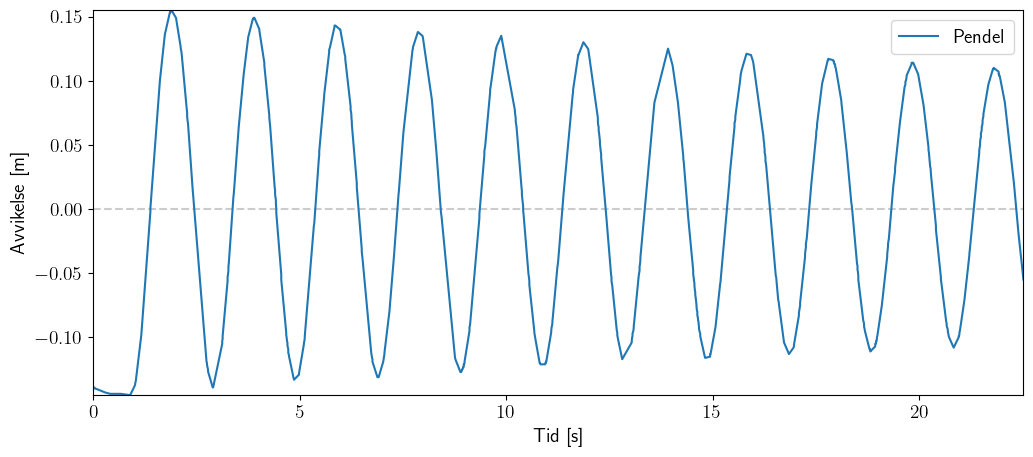
\includegraphics[width=\textwidth]{graf_egenfrekvens}
	\caption{Datan för svängning utan pålagd dämpning.}
	\label{fig:data_egenfrekvens}
\end{figure}

\begin{figure}[hp]
	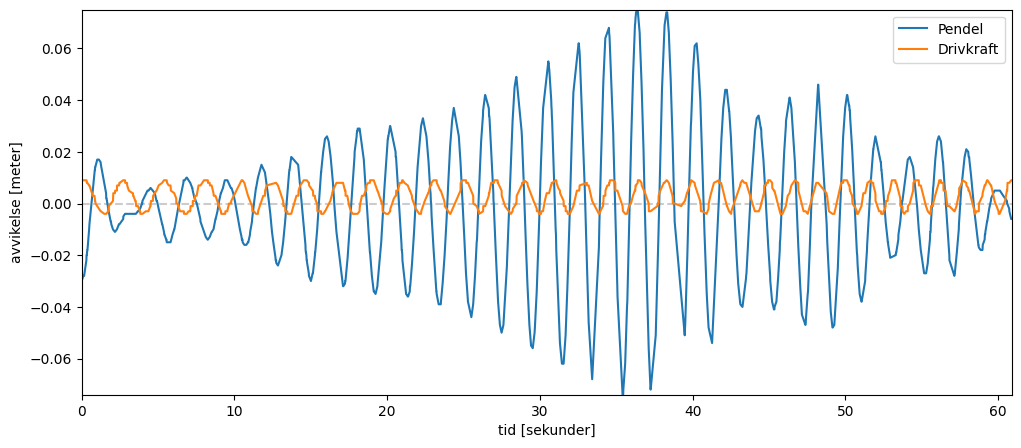
\includegraphics[width=\textwidth]{graf_resonansfrekvens}
	\caption{Datan för driven svängning runt resonansfrekvensen.}
	\label{fig:data_resonansfrekvens}
\end{figure}

\begin{figure}[hp]
	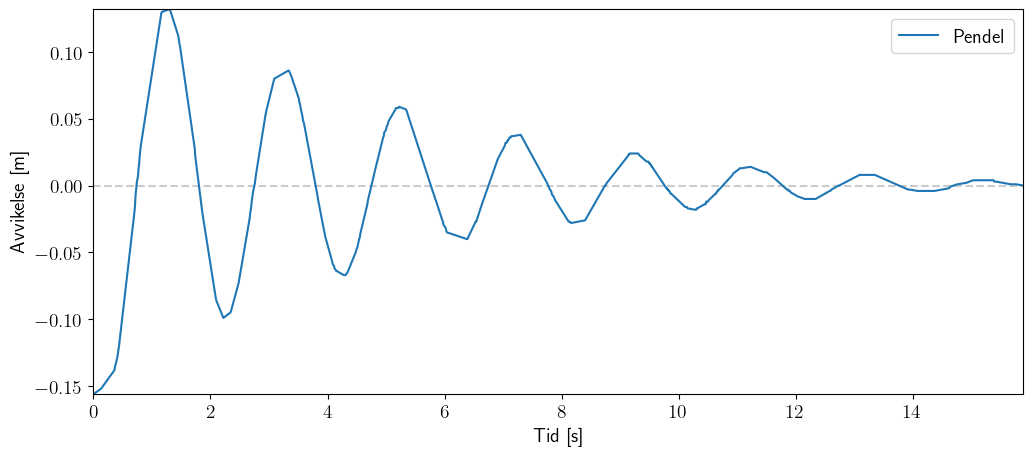
\includegraphics[width=\textwidth]{graf_1_v_centered}
	\caption{Datan för dämpad svängning med 1 V spänning i dämpningsenheten.}
	\label{fig:data_1_v}
\end{figure}

\begin{figure}[hp]
	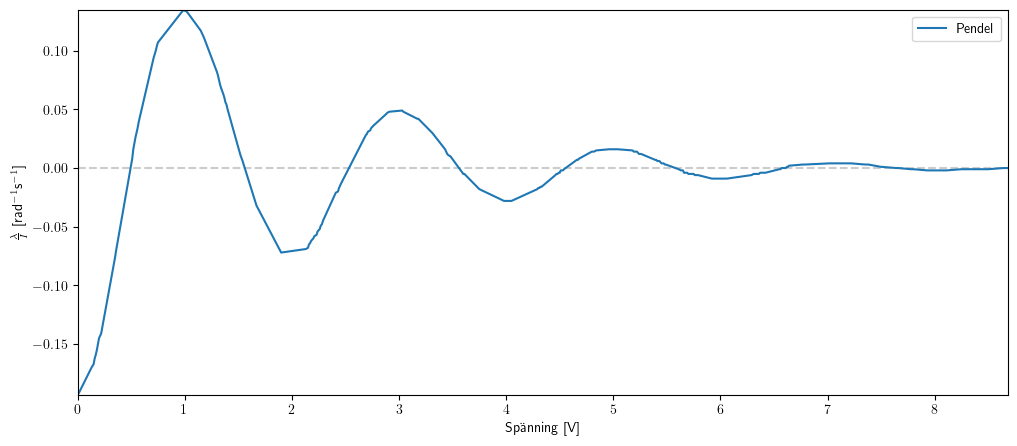
\includegraphics[width=\textwidth]{graf_4_v_centered}
	\caption{Datan för dämpad svängning med 4 V spänning i dämpningsenheten.}
	\label{fig:data_4_v}
\end{figure}

\begin{figure}[hp]
	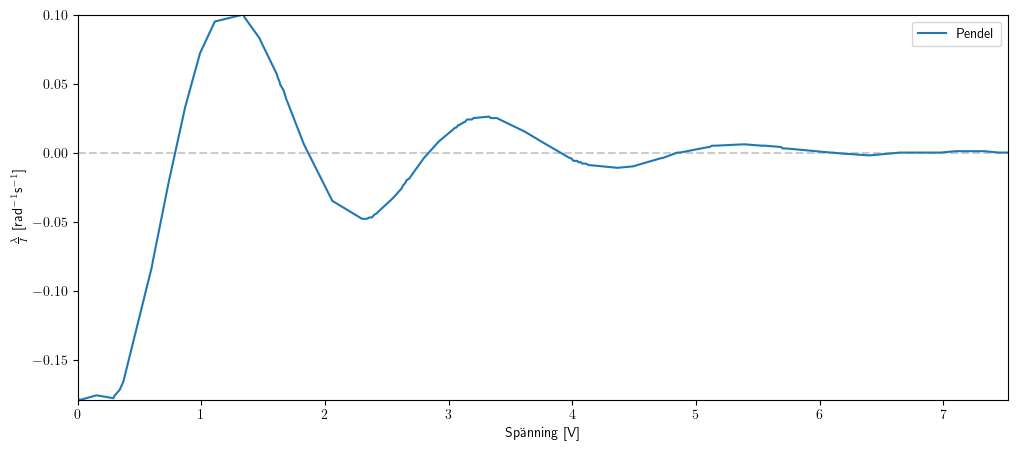
\includegraphics[width=\textwidth]{graf_5_v_centered}
	\caption{Datan för dämpad svängning med 5 V spänning i dämpningsenheten.}
	\label{fig:data_5_v}
\end{figure}

\begin{figure}[hp]
	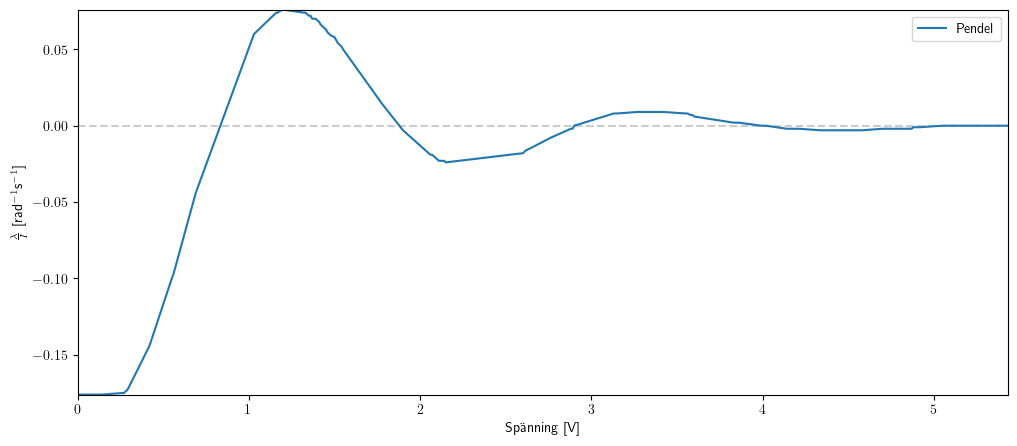
\includegraphics[width=\textwidth]{graf_6_v_centered}
	\caption{Datan för dämpad svängning med 6 V spänning i dämpningsenheten.}
	\label{fig:data_6_v}
\end{figure}

\begin{figure}[hp]
	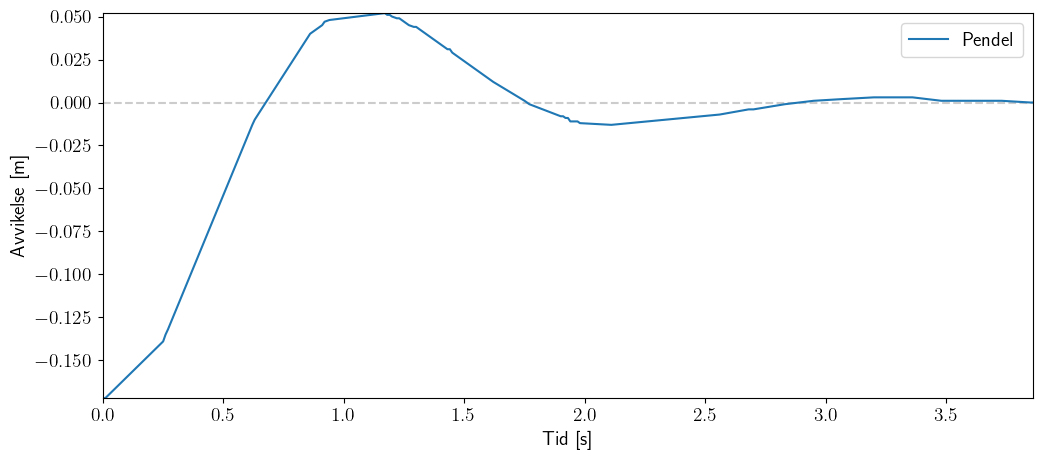
\includegraphics[width=\textwidth]{graf_7_v_centered}
	\caption{Datan för dämpad svängning med 7 V spänning i dämpningsenheten.}
	\label{fig:data_7_v}
\end{figure}

\begin{figure}[hp]
	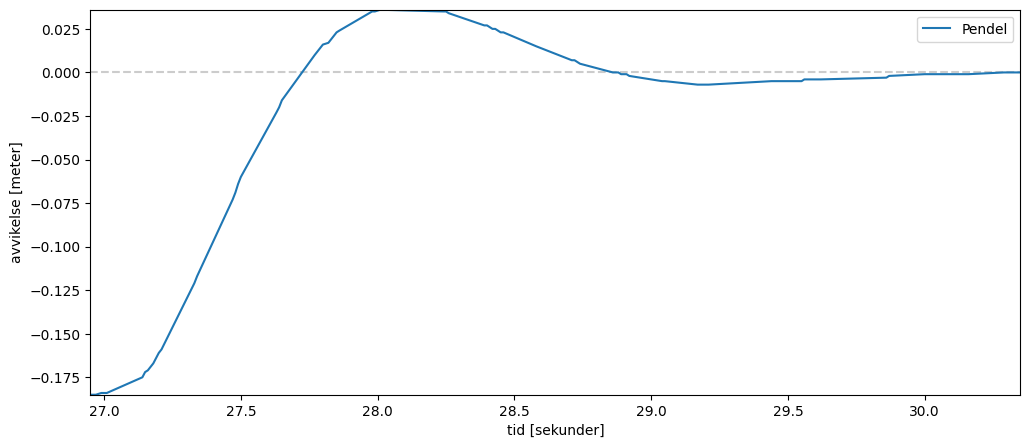
\includegraphics[width=\textwidth]{graf_8_v_centered}
	\caption{Datan för dämpad svängning med 8 V spänning i dämpningsenheten.}
	\label{fig:data_8_v}
\end{figure}

\begin{figure}[hp]
	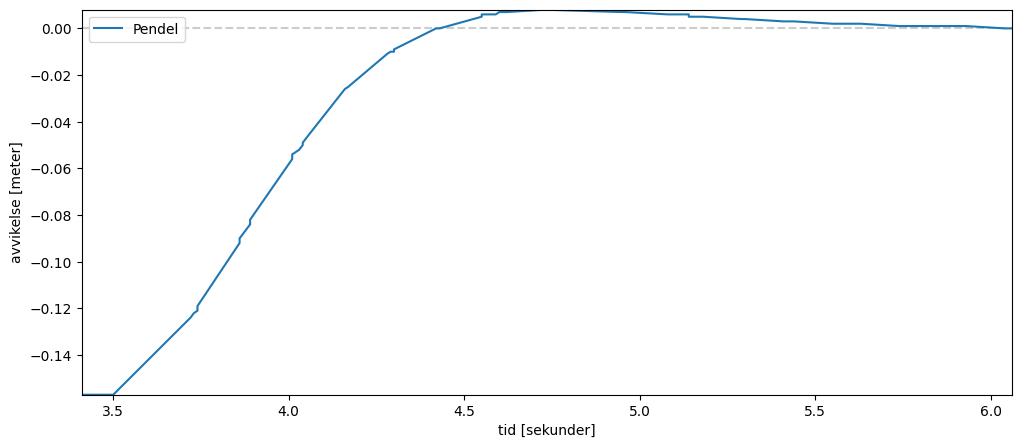
\includegraphics[width=\textwidth]{graf_9_v_centered}
	\caption{Datan för dämpad svängning med 9 V spänning i dämpningsenheten.}
	\label{fig:data_9_v}
\end{figure}

\begin{figure}[hp]
	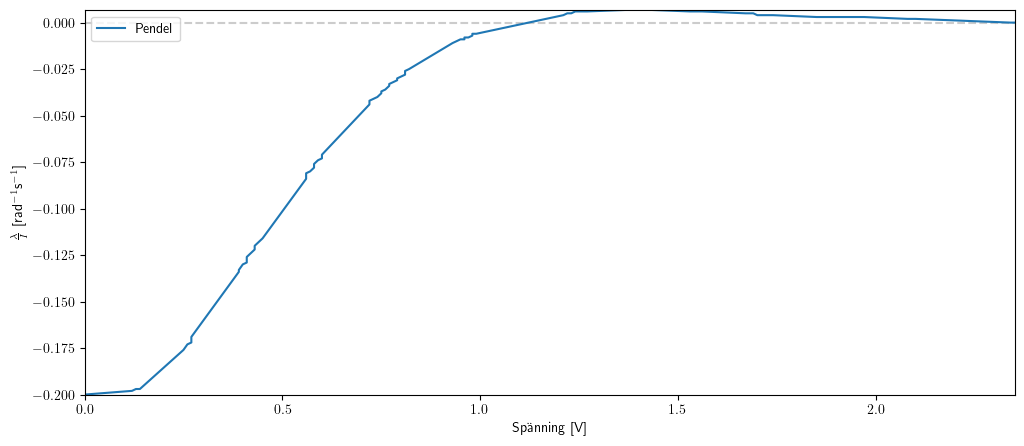
\includegraphics[width=\textwidth]{graf_10_v_centered}
	\caption{Datan för dämpad svängning med 10 V spänning i dämpningsenheten.}
	\label{fig:data_10_v}
\end{figure}

\begin{figure}[hp]
	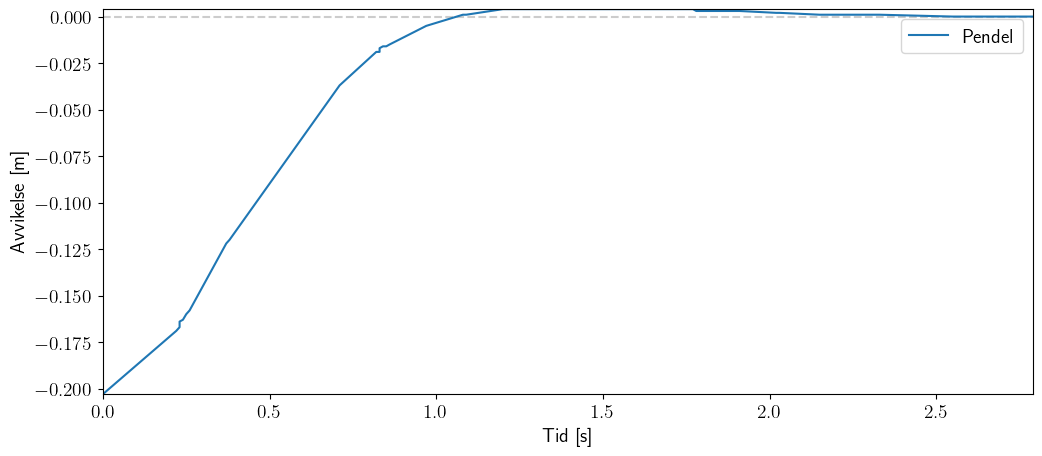
\includegraphics[width=\textwidth]{graf_11_v_centered}
	\caption{Datan för dämpad svängning med 11 V spänning i dämpningsenheten.}
	\label{fig:data_11_v}
\end{figure}

\begin{figure}[hp]
	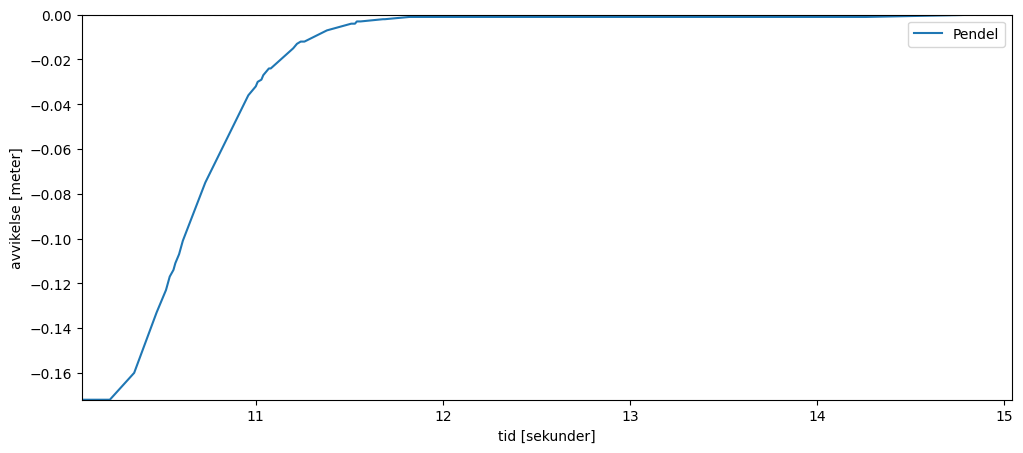
\includegraphics[width=\textwidth]{graf_13_v_centered}
	\caption{Datan för dämpad svängning med 13 V spänning i dämpningsenheten.}
	\label{fig:data_13_v}
\end{figure}

\begin{figure}[hp]
	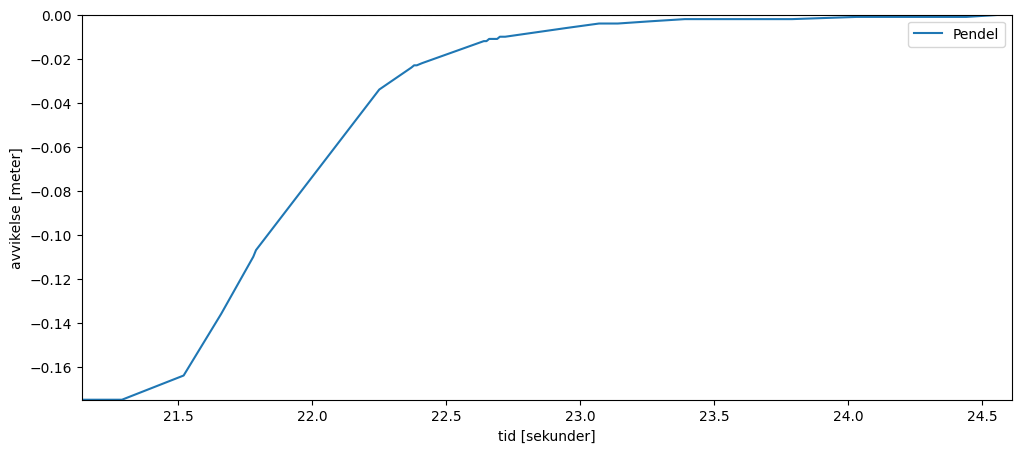
\includegraphics[width=\textwidth]{graf_14_v_centered}
	\caption{Datan för dämpad svängning med 14 V spänning i dämpningsenheten.}
	\label{fig:data_14_v}
\end{figure}

\clearpage
\section{Analys}
\subsection{Egenfrekvens}
Regressionsanalys av datan i figur \ref{fig:data_egenfrekvens} med lösningen i ekvation (\ref{eq:fri_pendel}) gav:
\begin{equation}
	\theta(t)=\frac{1}{r}0.125665\cdot\sin\bigl(3.15192t+1.81944\bigr)
\end{equation}
Med en determinationskoefficient $R^2\approx 98.92\%$.

Egenfrekvensen är alltså $\omega_0=\sqrt\frac{k}{I}=\SI{3.15192}{rad/s}$, amplituden $A=\SI{0.125665}{m}$, och fas\-förskjutningen $\phi=\SI{1.81944}{rad}$.

\subsection{Resonansfrekvens}
Regressionsanalys av drivenhetens läge (figur \ref{fig:data_resonansfrekvens}) i intervallet $t\in(30,36)$, strax innan pendelsvängningens amplitud var som störst, med lösningen i ekvation (\ref{eq:fri_pendel}) gav:
\begin{equation}
	y(t)=0.00631855\cdot\sin\bigl(3.35416t-1.75746\bigr)
\end{equation}
Med en determinationskoefficient $R^2\approx 96.57\%$ i området. Resonansfrekvensen som beräknades genom regressionen var alltså $\omega_r=\SI{3.35416}{rad/s}$. 

Ett annat sätt att beräkna resonansfrekvensen är med uttrycket i ekvation (\ref{eq:resonansfrekvens}). Utan någon dämpning i pendeln ger ekvationen $\omega_r=\omega_0$. Det finns dock ett litet luftmotstånd som dämpar pendeln naturligt, och denna ska enligt den matematiska modellen sänka resonansfrekvensen. Vi antar att även denna dämpningskraft är linjärt proportionell mot $\theta'(t)$.

Värdet på $\lambda$ kan inte beräknas utan att tröghetsmomentet $I$ för pendeln är känt. Endast förhållandet mellan $I$ och $\lambda$ kan hittas. Som tur är behöver bara $\frac{\lambda}{I}$ vara känt för att resonansfrekvensen ska kunna beräknas. Värdet på $\frac{\lambda}{I}$ i svängningen visad i figur \ref{fig:data_egenfrekvens} hittades genom regressionsanalys med uttrycket i ekvation (\ref{eq:svagt_dämpad}), med $\frac{\lambda}{I}$ substituerat mot en egen variabel $l$. Det resulterande värdet var $l\approx\SI{0.0316287}{rad^{-1}s^{-1}}$, med regressionens förklaringsgrad $R^2\approx 99.9\%$. Resonansfrekvensen blir då:
\begin{equation*}
	\omega_r=\sqrt{\omega_0^2-\frac{l^2}{2}}\approx\sqrt{3.15192^2-\frac{0.0316287^2}{2}}\approx\SI{3.15184}{rad/s}
\end{equation*}

Resonansfrekvensen beräknad från datan i figur \ref{fig:data_resonansfrekvens} är \SI{0.20224}{rad/s} större än torsionspendelns egenfrekvens och \SI{0.20232}{rad/s} större än resonansfrekvensen beräknad med ekvation (\ref{eq:resonansfrekvens}), vilket bryter mot den matematiska modellen eftersom resonansfrekvensen måste vara lägre än egenfrekvensen. 

Det kan finnas flera orsaker till detta. En skulle kunna vara brister i metoden, exempelvis att drivkraftens frekvens justerades kontinuerligt istället för stegvis. Det kan ha gjort att tidsintervallet som regressionsanalysen bör ha baserats på var otydligt. Det kan också ha gjort att modellen gav felaktiga resultat eftersom den antar att drivfrekvensen är konstant, trots att förändringen inte var särskilt hastig i experimentet.

\subsection{Dämpad svängning}
Figurerna \ref{fig:data_1_v}-\ref{fig:data_14_v}

\begin{table}[hp]
	\centering
	\begin{tabular}{ |l|l| }
		\hline 
		\rule{0ex}{1.5em}
		$U$ [V] & $\frac{\lambda}{I}$ [\si{rad^{-1}s^{-1}}]
		\\[0.5em]
		\hline
		0 & 0.032 \\
		\hline
		1 & 0.43 \\
		\hline
		4 & 0.96 \\
		\hline
		5 & 1.3 \\
		\hline
		6 & 1.7 \\
		\hline
		7 & 2.3 \\
		\hline
		8 & 2.9 \\
		\hline
		9 & 4.2 \\
		\hline
		10 & 4.3 \\
		\hline
		11 & 4.4 \\
		\hline
		13 & 5.1 \\
		\hline
		14 & 6.3 \\
		\hline
	\end{tabular}
	\caption{Avrundade värden på $\frac{\lambda}{I}$ för olika spänningsvärden i dämpningsenheten, framtagna med funktionsanpassning.}
\end{table}

\begin{figure}[hp]
	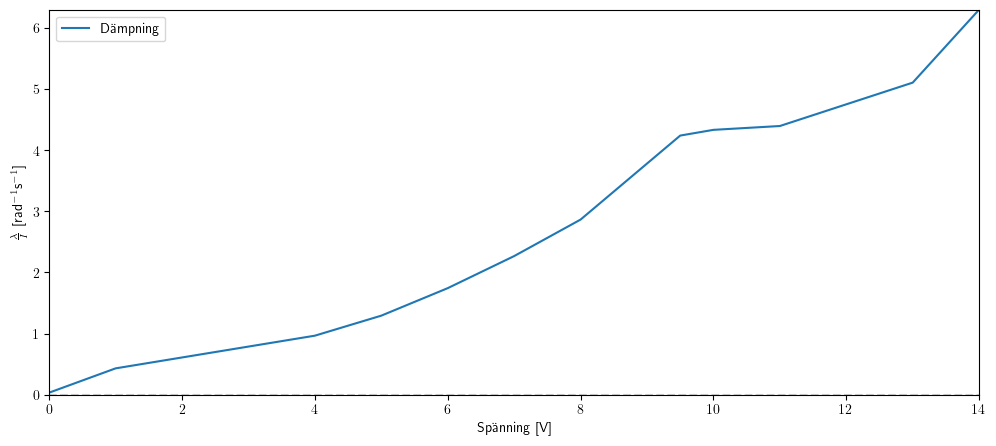
\includegraphics[width=\textwidth]{graf_voltage_damping}
	\caption{Graf av $\frac{\lambda}{I}$ över spänningen i dämpningsenheten med en linjär funktion och en potensfunktion anpassade till datan.}
	\label{fig:dämpning_över_spänning}
\end{figure}

\section{Slutsatser}

\end{document}